\documentclass[m3380-lec-main.tex]{subfiles}
\setcounter{chapter}{11}

%\DeclareMathOperator{\R}{\mathbb{R}}

\begin{document}


\chapter{Introduction to Graph Theory}

\section*{Goals}
\begin{enumerate}[1.~]\setlength{\itemsep}{0pt}
\item Define a \emph{graph}.
\item Discuss elementary properties of and definitions pertaining to graphs.
\item Discuss several different methods for representing graphs computationally.
\end{enumerate}

\section{Graphs}
\begin{defn} A \emph{graph} is an ordered pair $\Gamma=(V,E)$, where $V$ is a set of \emph{vertices} and $E$ is a set of \emph{edges}, where edges are unordered pairs of distinct vertices. That is, \[E \subseteq \set{\set{u,v}:u,v\in V}.\]
In order to simplify notation, we will write $uv$ instead of $\set{u,v}$ for an edge.
\end{defn}

\begin{rem} There are many, many different formulations for the definition of a graph. Some definitions are suffiently relaxed that an edge can loop back from a vertex to itself -- these are generally called \emph{loops}. Likewise, edges can be defined as independent objects with \emph{endpoints}, which allows for more than one edge to have vertices $u$ and $v$ as endpoints. I make the distinction that graphs which have loops or multiple edges are \emph{multipgraphs}. Some mathematicians are even more relaxed: their edges can contain more than two vertices, and the resulting structure is a \emph{hypergraph}!
\end{rem}

\begin{figure}[hbt]
\centerline{\begin{tikzpicture}
\draw \foreach \d/\c in {45/a, 135/b, 225/c, 315/d}{
    (\d:1) node[draw, circle={radius=1pt}, inner sep = 2pt] (\c) {}
    (\d:1.5) node {\c}
};
\draw (270:2) node {$K_4$};
\graph{ (a) -- {(b), (c), (d)}; (b) -- (c) -- (d) -- (b); };
\end{tikzpicture}
\qquad
{\fn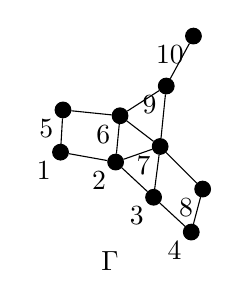
\begin{tikzpicture}[scale=1.5]
\draw 
(0.380612084622,-0.0802361442873) node [draw, fill=black, circle, inner sep = 2pt] (1) {}
(0.84723124048,-0.164013545485) node [draw, fill=black, circle, inner sep = 2pt] (2) {}
(1.16860759935,-0.462074965335) node [draw, fill=black, circle, inner sep = 2pt] (3) {}
(1.4877110863,-0.756751017894) node [draw, fill=black, circle, inner sep = 2pt] (4) {}
(0.401438801404,0.277296016838) node [draw, fill=black, circle, inner sep = 2pt] (5) {}
(0.884739088682,0.228005720311) node [draw, fill=black, circle, inner sep = 2pt] (6) {}
(1.22426111036,-0.0321294145258) node [draw, fill=black, circle, inner sep = 2pt] (7) {}
(1.58421317701,-0.392591983118) node [draw, fill=black, circle, inner sep = 2pt] (8) {}
(1.2759566434,0.479714229321) node [draw, fill=black, circle, inner sep = 2pt] (9) {}
(1.50619710517,0.902781104174) node [draw, fill=black, circle, inner sep = 2pt] (10) {};
\draw
(1) -- (2) (1) -- (5) (2) -- (3) (2) -- (6) (2) -- (7) (3) -- (4) (3) -- (7) (4) -- (8) (5) -- (6) (6) -- (7) (6) -- (9) (7) -- (8) (7) -- (9) (9) -- (10);
\draw \foreach \x in {1,...,10}{
    (\x) node [below left] {\x}
};
\draw (0.8,-1) node {\normalsize$\Gamma$};
\end{tikzpicture}}
\qquad
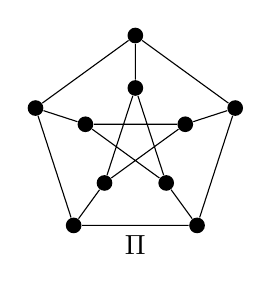
\begin{tikzpicture}[scale=2/3]
\draw \foreach \x in {1,...,5}{
    ({360*\x/5+18}:2) node [circle, fill=black, inner sep=2pt] (\x) {}
} (270:2) node {$\Pi$}
\foreach \x in {6,...,10}{
    ({360*(\x-5)/5+18}:1) node [circle, fill=black, inner sep = 2pt] (\x) {}
}
\foreach \x/\y/\z in {1/2/6, 2/3/7, 3/4/8, 4/5/9, 5/1/10}{
    (\x) -- (\y)
    (\x) -- (\z)
}
\foreach \x/\y in {6/8,7/9,8/10,9/6,10/7}{
    (\x) -- (\y)
};
\end{tikzpicture}}
\caption{Three graphs: $K_4$ is the \emph{complete graph} on 4 vertices and $\Pi$ is the \emph{Petersen graph}.}
\end{figure}

\subsection{Basic terminology}
\begin{defn} Two vertices $v_1,v_2\in V(\Gamma)$ are \emph{adjacent} if and only if $v_1v_2\in E(\Gamma)$. An edge $e\in E(\Gamma)$ is \emph{incident} with a vertex $v_1\in V(\Gamma)$ if and only if there is another vertex $v_2\in V(\Gamma)$ such that $v_1v_2 = e$.
\end{defn}
\begin{defn} The \emph{degree} of a vertex $v\in V(\Gamma)$ is the number of vertices adjacent to $v$; that is,
\[ d(v) = \abs{\set{u\in V:uv\in E}}. \]
\end{defn}

\begin{defn} A graph $\Gamma_1=(V_1, V_2)$ is a \emph{subgraph} of $\Gamma=(V,E)$ if and only if $V_1\subseteq V$ and $E_1\subseteq E$. $\Gamma_1$ is the \emph{subgraph of $\Gamma$ induced by $V_1$} if and only if $E_1 = \set{u_1v_1\in E: u_1,v_1\in V_1}$. That is, $\Gamma_1$ is an induced subgraph of $\Gamma$ if and only if every edge of $\Gamma$ between vertices of $\Gamma_1$ is an edge of $\Gamma_1$. There are many competing notations for induced subgraphs, but we will denote the induced subgraph of $V_1$ in $\Gamma$ by $\left\langle V_1\right\rangle_\Gamma$.
\end{defn}

\begin{figure}[hbt]\begin{center}\begin{tikzpicture}
\draw \foreach \x/\c/\d in {90/1/6, 162/2/7, 234/3/8, 306/4/9, 18/5/10}{
    (\x:2) node [circle, fill=black, inner sep=2pt] (\c) {}
    (\x:2.5) node {\c}
    (\x:1) node [circle, fill=black, inner sep=2pt] (\d) {}
    (\x+20:1) node {\d}
};
\graph[edges = {thick, red}]{(6) -- (8) -- (3) -- (4) -- (9) -- (6)};
\graph[edges = dashed]{
    (3) -- (2) -- (1) -- (5) -- (4)
    (2) -- (7) -- (10) -- (5)
    (1) -- (6)
    (7) -- (9) (10) -- (8)
};
\end{tikzpicture}\end{center}
\caption{The Petersen graph $\Pi$ and the subgraph induced by ${V_1=\set{v_3,v_4,v_6,v_8,v_9}}$. The edge set of $\vc{V_1}_\Pi$ is $E_1 = \set{v_3v_4, v_3v_8, v_4v_8, v_6v_8, v_6v_9}$, highlighted in red.}
\end{figure}


\begin{defn}\label{defn:isom} Two graphs $\Gamma=(V,E)$ and $\Gamma'=(V',E')$ are \emph{isomorphic} if there is a function $\phi:V\to V'$ such that the following three conditions hold. 
\begin{enum}
\item (Injective) If $v_1,v_2\in V$ with $v_1\neq v_2$, then $\phi(v_1)\neq\phi(v_2)$.
\item (Surjective) If $v'\in V'$, then there is some $v\in V$ such that $\phi(v)=v'$.
\item (Graph Homomorphism) $v_1v_2\in E$ if and only if $v_1'v_2'\in E'$, where $\phi(v_1)=v_1'$ and $\phi(v_2)=v_2'$.
\end{enum}
If such a function exists, we write $\Gamma\cong \Gamma'$.
\end{defn}
Each of these conditions independently are important, but their combination is essential in graph theory: a graph isomorphism is an \emph{adjacency-preserving bijection between vertex sets}.

\begin{defn} Let $\Gamma=(V,E)$. A permutation $\phi:V\to V$ which satisfies condition (3) of Definition \ref{defn:isom}{} is a \emph{graph automorphism}. The set of all automorphisms of a graph $\Gamma$ is denoted $\Aut\Gamma$.
\end{defn}

\begin{figure}[hbt]
\begin{center}
\begin{tikzpicture}
\draw \foreach \x/\c in {45/a,135/b,225/c,315/d}{
    (\x:1) node [draw, circle={radius=1pt}, inner sep = 2pt] (\c) {}
    (\x:1.5) node {$\c$}
};
\graph{ (a) -- {(b), (c), (d)}; (b) -- (c) -- (d) -- (b); };
\node at (0,-2) {$K_4$};
\end{tikzpicture} \hspace{2cm}
\begin{tikzpicture}
\draw \foreach \x/\b/\c in {90/b/$v_2$, 210/c/$v_3$, 330/d/$v_4$}{
    (\x:1) node [draw, circle={radius=1pt}, inner sep = 2pt] (\b) {}
    (\x:1.5) node {\c}
};
\node [draw, circle={radius=1pt}, inner sep=2pt] at (0,0) (a) {};
\node [below=2pt] at (a) {$v_1$};
\graph{ (a) -- {(b), (c), (d)}; (b) -- (c) -- (d) -- (b); };
\node at (0,-2) {$K'_4$};
\end{tikzpicture}
\end{center}
\caption{While $K_4\neq K'_4$, the two graphs are isomorphic. In fact, since these are \emph{complete} graphs, every bijection between the sets $\set{a,b,c,d}$ and $\set{v_1,v_2,v_3,v_4}$ is an isomorphism.}
\end{figure}

\begin{defn} Suppose $\Gamma=(V,E)$ is a graph and $u,v\in V$. A \emph{path} between $u$ and $v$ is any sequence 
\[ (u=v_0, e_1, v_1, e_2, v_2, \ldots, v_{n-1}, e_n, v_n = v)\]
such that $e_i = v_{i-1}v_i$ for each $i\in\set{1,2,\ldots,n}$ and $v_i\neq v_j$ if $i\neq j$. This can also be called a \emph{$u,v$-path}. A path containing $n$ edges is a path of \emph{length} $n$.
\end{defn}

\begin{defn} Let $\Gamma=(V,E)$ be a graph and $v_1, v_2\in V$. The \emph{distance from $v_1$ to $v_2$} is the length of a shortest path between $v_1$ and $v_2$. If no such path exists, the distance from $v_1$ to $v_2$ is $\infty$. Distance between $v_1$ and $v_2$ in the graph $\Gamma$ is sometimes denoted $d_\Gamma(v_1,v_2)$, which can be easily confused with the notation for degree.
\end{defn}

\begin{defn}
A \emph{cycle} is a sequence 
\[ (v_0,e_1,v_1, e_2, v_2, \ldots, v_{n-1}, e_n, v_n = v_0)\]
such that $e_i = v_{i-1}v_i$ for each $i\in\set{1,2,\ldots,n}$ and $v_i\neq v_j$ if $i\neq j$ except for $v_0=v_n$. A cycle containing $n$ edges is an $n$-cycle, and is isomorphic to the cycle graph $C_n=(\mathbb{Z}_n, \set{ab:a,b\in\mathbb{Z}_n, a-b\equiv 1\mod(n)}$.
\end{defn}

\begin{figure}[hbt]
\begin{center}\begin{tikzpicture}
\draw \foreach \x/\c/\d in {90/1/6, 162/2/7, 234/3/8, 306/4/9, 18/5/10}{
    (\x:2) node [circle, fill=black, inner sep=2pt] (\c) {}
    (\x:2.5) node {\c}
    (\x:1) node [circle, fill=black, inner sep=2pt] (\d) {}
    (\x+20:1) node {\d}
};
\graph[edges = {red, thick}]{(1) -- (6) -- (8) -- (3)};
\graph[edges = {blue, thick}]{
    (1) -- (2) -- (7) -- (10) -- (5) -- (4) -- (3)
};
\graph[edges = dashed]{
    (1) -- (5) (2) -- (3) (8) -- (10)
    (9) -- {(4), (6), (7)}
};
\end{tikzpicture}
\end{center}
\caption{The Petersen graph with two distinct (and openly disjoint) $v_1,v_3$-paths, one highlighted in red and the other in blue. The union of the red and blue paths is a 9-cycle in $\Pi$.}
\end{figure}

\begin{defn}
The graph $\Gamma$ is \emph{connected} if and only if for any two distinct vertices $v_1,v_2\in V$ there is at least one $v_1,v_2$-path.
\end{defn}

\begin{defn} A subgraph $\Gamma_=(V_1,E_2)$ of a graph $\Gamma=(V,E)$ is a \emph{component} of $\Gamma$ if and only if $\Gamma_1=\vc{V_1}_\Gamma$ and $\vc{V_1\cup\set{u}}_\Gamma$ is disconnected for any vertex $u\in V\setminus V_1$. Clearly, a connected graph has only one component.
\end{defn}

\begin{defn} A connected graph containing no cycles is called a \emph{tree}. An arbitrary graph containing no cycles is called a \emph{forest}. For a given graph $\Gamma=(V,E)$, a forest $\Phi=(V,E')$ where $E'\subseteq E$ is called a \emph{spanning forest}. A \emph{spanning tree} of a connected graph is defined analogously.
\end{defn}

These are just a few of the ``basic definitions" of graph theory. It is a subject which is very appealing for research as the problems are often visually interesting. Since problems in the field are very accessible, some mathematicians are mildly derogatory towards graph theory, calling the field ``recreational mathematics." If that is so, then the vast number of graph theorists are perhaps the luckiest of all mathematicians: their chosen field of research is seen to be fun and games by their colleagues!

All joking aside, graph theory and the larger discipline of combinatorics are deeply applicable fields. There are many ``real world" problems which are modeled by discrete systems (rather than continuous systems such as used in differential equations or traditional applied math courses), and graph theory techniques are often the best solution to these problems. So while combinatorics is not generally considered part of applied mathematics, it is very \emph{applicable} mathematics.

\section{Representing graphs computationally}
There are many problems in discrete modeling which are best solved using graph theory, so it is important to be able to represent graphs as some sort of data structure. In fact, there is an abstract data structure called a graph! This data structure is often of limited use when trying to solve mathematical problems on graphs, so we will focus instead on other methods of implementing graphs.

We will begin with a representation that is easily understandable and build towards representations that provide more theoretical power.

\subsection{Edge lists}
The simplest way to represent a graph is to provide a list of the vertices and the edges; while the edges can be stored either as lists or tuples, we will prefer tuples so they are immutable. We'll consider again the Petersen graph, this time with vertices labeled from $0$ through $9$.

\begin{figure}[hbt]
\begin{center}\begin{tikzpicture}
\draw \foreach \x/\c/\d in {90/0/5, 162/1/6, 234/2/7, 306/3/8, 18/4/9}{
    (\x:2) node [circle, fill=black, inner sep=2pt] (\c) {}
    (\x:2.5) node {\c}
    (\x:1) node [circle, fill=black, inner sep=2pt] (\d) {}
    (\x+20:1) node {\d}
};
\graph{
(0) -- {(1) -- {(2) -- {(7)--(9), (3)--(8)}, (6)--{(8), (9)}}, (4) -- {(3), (9)}, (5) -- {(7), (8)}}
};
\end{tikzpicture}
\end{center}
\caption{The Petersen graph with vertices $V=\set{v_0,v_1,\ldots,v_9}$.}
\end{figure}

In Python, the list of edges can be given using the integer indices of vertices as the ``name" of the vertex. So the vertex list and list of edges as tuples are as given below:

\bc
\begin{verbatim}
V = list(range(10))
E = [(0, 1), (0, 4), (0, 5), (1, 2), (1, 6), (2, 3), (2, 7), (3, 4), (3, 8), 
     (4, 9), (5, 7), (5, 8), (6, 8), (6, 9), (7, 9)]
\end{verbatim}
\ec

We notice that each edge is listed only once, in one direction -- algorithms must take this into account! Even though $v_0v_1$ is the same edge as $v_1v_0$, there are often times when we will want to use the edge in the latter order rather than the former. This makes an edge list slightly less useful than some of the other representations when we move into implementing algorithms.

Equivalent to an edge list is an edge dictionary: the dictionary representation of this edge list is 

\bc
\begin{verbatim}
d = {0: [1, 4, 5], 1: [2, 6], 2: [3, 7], 3: [4, 8], 4: [9], 5: [7, 8], 6: [8, 9],
     7: [9]}
\end{verbatim}
\ec
This suffers from exactly the same limitation as the edge list. A simple solution is to use a ``double-ended" dictionary:

\bc
\begin{verbatim}
ded = {0: [1, 4, 5], 1: [0, 2, 6], 2: [1, 3, 7], 3: [2, 4, 8], 4: [0, 3, 9],
       5: [0, 7, 8], 6: [1, 8, 9], 7: [2, 5, 9], 8: [3, 5, 6], 9: [4, 6, 7]}
\end{verbatim}
\ec
While this stores every edge twice, it allows us to access each edge from either endpoint.

\subsection{Adjacency matrices}
From the idea of a double-ended edge dictionary it is a small step to build the adjacency matrix of a graph. 

\begin{defn} Suppose $\Gamma=(V,E)$ is a graph with vertices $V=\set{v_0,v_1,\ldots, v_{n-1}}$. Then the \emph{adjacency matrix} of $\Gamma$ is the $n\times n$ matrix $A=[a_{i,j}]$ with
\[a_{i,j} = \begin{cases}1 & v_iv_j\in E \\ 0 & v_iv_j\notin E \end{cases}.\]
\end{defn}

The adjacency matrix of the Petersen graph as above is 
{\fn \[ A = \begin{bmr}
0 & 1 & 0 & 0 & 1 & 1 & 0 & 0 & 0 & 0 \\
1 & 0 & 1 & 0 & 0 & 0 & 1 & 0 & 0 & 0 \\
0 & 1 & 0 & 1 & 0 & 0 & 0 & 1 & 0 & 0 \\
0 & 0 & 1 & 0 & 1 & 0 & 0 & 0 & 1 & 0 \\
1 & 0 & 0 & 1 & 0 & 0 & 0 & 0 & 0 & 1 \\
1 & 0 & 0 & 0 & 0 & 0 & 0 & 1 & 1 & 0 \\
0 & 1 & 0 & 0 & 0 & 0 & 0 & 0 & 1 & 1 \\
0 & 0 & 1 & 0 & 0 & 1 & 0 & 0 & 0 & 1 \\
0 & 0 & 0 & 1 & 0 & 1 & 1 & 0 & 0 & 0 \\
0 & 0 & 0 & 0 & 1 & 0 & 1 & 1 & 0 & 0
\end{bmr}\].}
If we have the double-ended dictionary stored as \verb|ded| and the vertex list as \verb|V|, we can create this adjacency matrix easily using a list comprehension:

\bc
\begin{verbatim}
A = [[1 if v in ded[u] else 0 for v in V] for u in V]
\end{verbatim}
\ec

\end{document}
